\documentclass[11pt]{article}
\usepackage{amsmath,amssymb,amsthm}
\usepackage{graphicx}
\usepackage[margin=1in]{geometry}

\graphicspath{{../blocks/}}

\newtheorem{definition}{Definition}
\newtheorem{theorem}{Theorem}
\newtheorem{example}{Example}
\newtheorem{remark}{Remark}

\title{Central-Potential Scattering, the Rutherford Cross Section,\\
and Hamiltonian Mechanics}
\author{HC 6001 --- Classical Mechanics}
\date{October 22, 2024}

\begin{document}
\maketitle

\section{Scattering by a central potential --- setup}

% block_001 | content_type: definition | confidence: high
\begin{definition}[Scattering by a central potential]
Consider a beam of particles scattered by a central potential $V(r)$. The incident
energy and velocity are
\begin{equation}
  E = \frac{m}{2} v_0^2, \qquad v_0 = \sqrt{\frac{2E}{m}}.
\end{equation}
The orbital angular momentum is fixed by the impact parameter $s$,
\begin{equation}
  l = m s v_0 = s\sqrt{2mE}, \qquad s = \frac{l}{\sqrt{2mE}}.
\end{equation}
In spherical coordinates the volume element is $d^3r = r^2\,dr\,d\Omega$ with
$d\Omega = \sin\theta\,d\theta\,d\phi$. Because the azimuthal angle $\phi$ is irrelevant
by symmetry, the solid-angle element for scattering into deflection angle $\theta$ is
\begin{equation}
  d\Omega = 2\pi\sin\theta\,d\theta.
\end{equation}
\end{definition}

\begin{figure}[htbp]
  \centering
  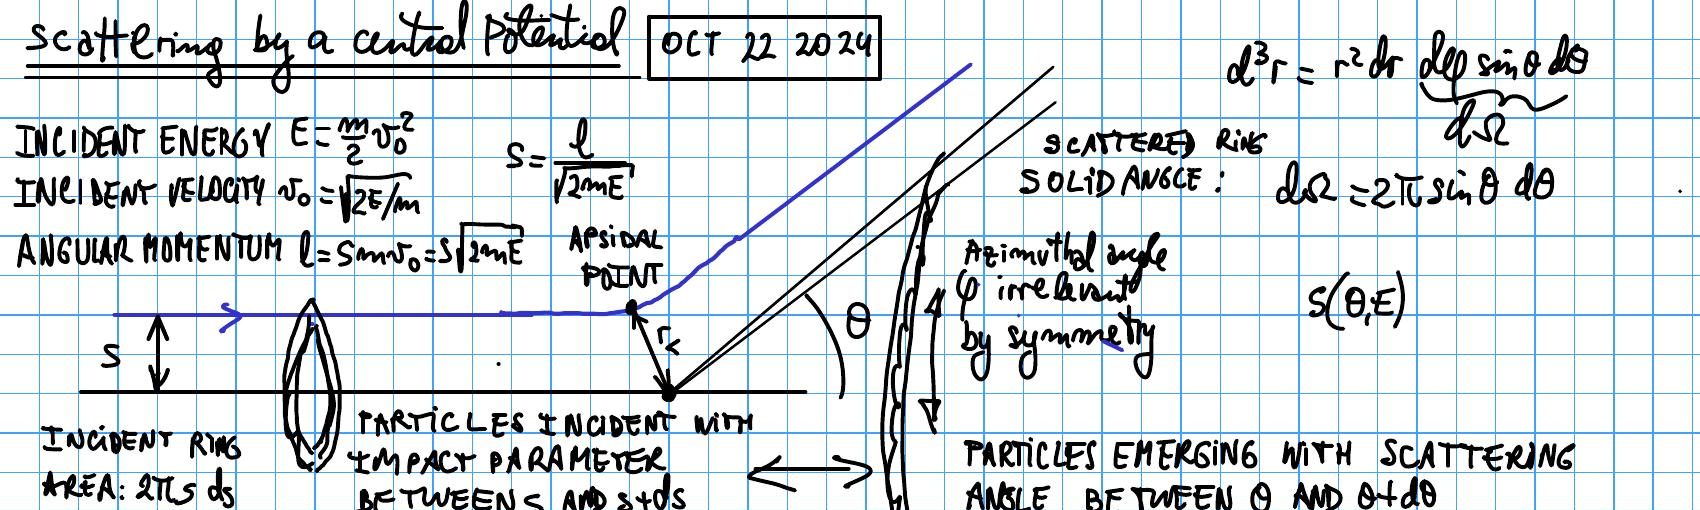
\includegraphics[width=0.95\textwidth]{block_001/image.png}
  \caption{Scattering trajectory: impact parameter $s$, apsidal point at $r_c$, and
  deflection angle $\theta$; particles incident in the ring between $s$ and $s+ds$ emerge
  between $\theta$ and $\theta+d\theta$.}
\end{figure}

\section{Incident intensity and differential cross section}

% block_002 | content_type: derivation | confidence: high | depends_on: block_001
Let the incident intensity $I$ be the number of particles incident per unit time per unit
beam cross-sectional area. The differential cross section $\sigma(\Omega)$ is defined by
\begin{equation}
  \sigma(\Omega)\,d\Omega
  = \frac{\text{\# particles scattered into } d\Omega \text{ per unit time}}{I}.
\end{equation}
Particles incident through the ring between impact parameters $s$ and $s+ds$ occupy area
$2\pi s\,|ds|$ and emerge with deflection angle between $\theta$ and $\theta+d\theta$.
Conservation of particle number gives
\begin{equation}
  I\,(2\pi s)\,|ds| = I\,\sigma(\theta)\,2\pi\sin\theta\,|d\theta|,
\end{equation}
so that
\begin{equation}
  \sigma(\theta) = \frac{s}{\sin\theta}\left|\frac{ds}{d\theta}\right|.
  \label{eq:sigma-theta}
\end{equation}
The total cross section is
\begin{equation}
  \sigma_T = \int d\Omega\,\sigma(\Omega).
\end{equation}

\section{Repulsive vs.\ attractive scattering geometry}

% block_003 | content_type: diagram | confidence: high | depends_on: block_001
Let $\psi$ be the angle between the incident asymptote (the horizontal) and the apsidal
direction. The geometry relates $\psi$ to the deflection angle $\theta$ differently in the
two cases:
\begin{align}
  \text{repulsive:}  \quad & \theta = \pi - 2\psi, & \psi &= \frac{\pi-\theta}{2}, \\
  \text{attractive:} \quad & \theta = 2\psi - \pi, & \psi &= \frac{\pi+\theta}{2},
\end{align}
and in all cases
\begin{equation}
  \theta = \lvert\,\pi - 2\psi\,\rvert.
\end{equation}

\begin{figure}[htbp]
  \centering
  
\includegraphics[width=0.95\textwidth]{block_003/image.png}
  \caption{Repulsive (left) and attractive (right) central-potential trajectories, showing
  the apsidal point and the angle $\psi$ to the horizontal.}
\end{figure}

\section{Universal scattering-angle integral for any $V(r)$}

% block_004 | content_type: derivation | confidence: high | depends_on: block_001, block_003
To obtain $s(\theta,E)$ for an arbitrary central potential, begin from energy conservation
including the centrifugal term,
\begin{equation}
  E = \frac{m}{2}\dot{r}^2 + V(r) + \frac{l^2}{2mr^2}.
\end{equation}
Solving for the radial velocity,
\begin{equation}
  \dot{r} = \left[\frac{2}{m}\left(E - V(r) - \frac{l^2}{2mr^2}\right)\right]^{1/2},
  \qquad dt = \frac{dr}{\dot{r}}.
\end{equation}
With $l = mr^2\dot{\theta}$ we have $\dot{\theta} = l/(mr^2)$, hence
\begin{equation}
  d\theta = \dot{\theta}\,dt = \frac{l}{mr^2}\,dt
  = \frac{l\,r^{-2}\,dr}
         {\sqrt{2m\left(E - V(r) - \dfrac{l^2}{2mr^2}\right)}}.
\end{equation}
Substituting $l = s\sqrt{2mE}$ and dividing through by $E$,
\begin{equation}
  d\theta = \frac{s\,r^{-2}\,dr}{\sqrt{1 - \dfrac{V(r)}{E} - \dfrac{s^2}{r^2}}}.
\end{equation}
Integrating from the distance of closest approach $r_m$ to infinity gives the apsidal
angle
\begin{equation}
  \psi = \int_{r_m}^{\infty}
  \frac{s\,r^{-2}\,dr}{\sqrt{1 - \dfrac{V(r)}{E} - \dfrac{s^2}{r^2}}}.
\end{equation}
With the substitution $u = 1/r$, $du = -r^{-2}\,dr$, and $u_m = 1/r_m$,
\begin{equation}
  \psi = \int_0^{u_m}
  \frac{s\,du}{\sqrt{1 - \dfrac{V(u)}{E} - s^2 u^2}}.
\end{equation}

% block_005 | content_type: equation | confidence: high | depends_on: block_004
Using $\theta = |\pi - 2\psi|$, the scattering angle for any central potential is
\begin{equation}
  \theta(s) = \left\lvert\,
  \pi - 2\int_0^{u_m}
  \frac{s\,du}{\sqrt{1 - \dfrac{V(u)}{E} - s^2 u^2}}
  \,\right\rvert.
  \label{eq:theta-universal}
\end{equation}
From $\theta(s)$ one obtains $\lvert ds/d\theta\rvert = 1/\lvert d\theta/ds\rvert$ and hence
$\sigma(\theta)$ through \eqref{eq:sigma-theta}.
\textbf{Up to this point every result is valid for any central potential $V(r)$.}

\section{Coulomb scattering --- hyperbolic orbits and eccentricity}

% block_006 | content_type: definition | confidence: high | depends_on: block_005
\begin{definition}[Coulomb scattering]
For the Coulomb interaction the force and potential are
\begin{equation}
  f = \frac{ZZ'e^2}{r^2}, \qquad V(r) = -\frac{k}{r}, \qquad k = -ZZ'e^2.
\end{equation}
For $V = -k/r$ \emph{only}, the orbit type is set by the sign of the energy:
\begin{itemize}
  \item $E > 0$: hyperbolic orbit (scattering),
  \item $E = 0$: parabolic orbit,
  \item $E < 0$: elliptic orbit.
\end{itemize}
\end{definition}

% block_007 | content_type: derivation | confidence: high | depends_on: block_006
For scattering ($E > 0$) the orbit equation is
\begin{equation}
  \frac{1}{r} = C\bigl[1 + \epsilon\cos(\theta - \theta')\bigr],
\end{equation}
with coefficient and eccentricity
\begin{equation}
  C = \frac{mk}{l^2}, \qquad
  \epsilon = \left[1 + \frac{2El^2}{mk^2}\right]^{1/2}
           = \left[1 + \left(\frac{2sE}{ZZ'e^2}\right)^2\right]^{1/2} > 1,
\end{equation}
where $l = s\sqrt{2mE}$ was used. Two physically distinct situations arise:
\begin{itemize}
  \item[i)] \textbf{repulsive}: $ZZ' > 0 \Rightarrow k = -ZZ'e^2 < 0$;
  \item[ii)] \textbf{attractive}: $ZZ' < 0 \Rightarrow k > 0$ (also gravity, $k = Gm_1m_2$).
\end{itemize}

\section{Coulomb scattering --- repulsive case}

% block_008 | content_type: derivation | confidence: high | depends_on: block_007
\textbf{Case i (repulsive):} here $k < 0$, so $C = mk/l^2 < 0$. Positivity of $1/r$
requires
\begin{equation}
  1 + \epsilon\cos(\theta - \theta') < 0
  \quad\Longleftrightarrow\quad
  \cos(\theta - \theta') < -\frac{1}{\epsilon},
\end{equation}
so $\theta - \theta' = 0$ lies inside the inaccessible region and periapsis occurs at
$\theta' = \pi$. Using $\cos(\theta - \pi) = -\cos\theta$,
\begin{equation}
  \frac{1}{r} = \frac{mZZ'e^2}{l^2}\bigl(\epsilon\cos\theta - 1\bigr),
\end{equation}
which is maximal (radius minimal) at the apsidal point $\theta = 0$,
\begin{equation}
  \frac{1}{r_m} = \frac{mZZ'e^2}{l^2}\,(\epsilon - 1).
\end{equation}
As $r \to \infty$ the bracket vanishes, giving $\cos\psi = 1/\epsilon$. With
$\psi = (\pi - \theta)/2$,
\begin{equation}
  \frac{1}{\epsilon} = \cos\frac{\pi-\theta}{2} = \sin\frac{\theta}{2}.
\end{equation}

\section{Coulomb scattering --- attractive case}

% block_009 | content_type: derivation | confidence: high | depends_on: block_007
\textbf{Case ii (attractive):} here $k > 0$, so $C = km/l^2 > 0$. Take $\theta' = 0$, so
\begin{equation}
  \frac{1}{r} = C\bigl[1 + \epsilon\cos\theta\bigr],
\end{equation}
maximal at the apsidal point $\theta = 0$. As $r \to \infty$, $\cos\psi = -1/\epsilon$.
With $\psi = (\pi + \theta)/2$,
\begin{equation}
  -\frac{1}{\epsilon} = \cos\frac{\pi+\theta}{2} = -\sin\frac{\theta}{2}
  \quad\Longrightarrow\quad
  \frac{1}{\epsilon} = \sin\frac{\theta}{2},
\end{equation}
identical to the repulsive relation.

\section{Rutherford differential cross section}

% block_010 | content_type: derivation | confidence: high | depends_on: block_008, block_009
Combining both cases through $1/\epsilon = \sin(\theta/2)$,
\begin{equation}
  \cot^2\frac{\theta}{2}
  = \frac{1}{\sin^2\frac{\theta}{2}} - 1
  = \epsilon^2 - 1
  = \left(\frac{2sE}{ZZ'e^2}\right)^2,
\end{equation}
so the impact parameter as a function of angle is
\begin{equation}
  s(\theta,E) = \left\lvert\frac{ZZ'e^2}{2E}\right\rvert\cot\frac{\theta}{2}.
\end{equation}
Differentiating,
\begin{equation}
  \frac{ds}{d\theta}
  = -\left\lvert\frac{ZZ'e^2}{2E}\right\rvert\frac{1}{2\sin^2\frac{\theta}{2}}
  = -\left\lvert\frac{ZZ'e^2}{4E}\right\rvert\frac{1}{\sin^2\frac{\theta}{2}},
\end{equation}
and substituting into \eqref{eq:sigma-theta} with $\sin\theta = 2\sin(\theta/2)\cos(\theta/2)$,
\begin{equation}
  \sigma(\theta) = \frac{1}{4}\left(\frac{ZZ'e^2}{2E}\right)^2
  \csc^4\frac{\theta}{2}.
  \label{eq:rutherford}
\end{equation}
This is the \textbf{Rutherford scattering cross section} for the Coulomb force.

% block_011 | content_type: remark | confidence: high | depends_on: block_010
\begin{remark}[Properties of the Rutherford cross section]
\begin{enumerate}
  \item It is the same for the repulsive and attractive cases, since it depends only on
  $(ZZ')^2$.
  \item It diverges like $E^{-2}$ at low incident energies.
  \item It diverges like $\theta^{-4}$ (very strongly) at small scattering angles.
  \item The classical result is exactly the same as the quantum-mechanical result.
\end{enumerate}
\end{remark}

% block_012 | content_type: derivation | confidence: high | depends_on: block_010
The total cross section is
\begin{equation}
  \sigma_T = \int \sigma(\Omega)\,d\Omega,
  \qquad \sigma(\theta) = \text{const}\times\frac{1}{\sin^4\frac{\theta}{2}}.
\end{equation}
Writing $d\Omega = 2\pi\sin\theta\,d\theta = 4\pi\sin\frac{\theta}{2}\cos\frac{\theta}{2}\,d\theta$,
\begin{equation}
  \sigma_T = \frac{4\pi}{4}\left(\frac{ZZ'e^2}{2E}\right)^2
  \int_0^{\pi}\frac{\sin\frac{\theta}{2}\cos\frac{\theta}{2}}{\sin^4\frac{\theta}{2}}\,d\theta
  \;\sim\; \int_0 \frac{d\theta}{(\theta/2)^3}
  = 8\int_0 \frac{d\theta}{\theta^3},
\end{equation}
whose lower limit behaves like $\theta^{-2}\big|_0 \to +\infty$. Hence $\sigma_T$ is
\textbf{strongly divergent}.

\section{Notation, divergent total cross section, screened potentials}

% block_013 | content_type: remark | confidence: high | depends_on: block_012
\begin{remark}[Notation and long-range potentials]
Goldstein writes $\sigma(\Omega)$ and $\sigma_T$ for the differential and total cross
sections, where other texts write $d\sigma/d\Omega$ and $\sigma$, respectively.

Classically, $\sigma_T = +\infty$ for \emph{any} long-range potential. Quantum
mechanically, $\sigma_T = +\infty$ only for some long-range potentials $V(r)$ that do not
decay fast enough as $r \to \infty$.

\textbf{Caveat:} in a dense conducting material the Coulomb potential becomes a screened
(Yukawa) potential,
\begin{equation}
  V_{\mathrm{screen}}(r) = -\frac{k}{r}\,e^{-r/\lambda}.
\end{equation}
In non-conducting materials the screened potential may take a different form but still
vanishes much faster than $1/r$, rendering $\sigma_T$ finite.
\end{remark}

\begin{figure}[htbp]
  \centering
  
\includegraphics[width=0.85\textwidth]{block_013/image.png}
  \caption{Scattering-center geometry, notation comparison, and the screened Coulomb
  (Yukawa) caveat (from the lecture notes).}
\end{figure}

\section{Hamiltonian mechanics --- Lagrangian review}

% block_014 | content_type: definition | confidence: high
\begin{definition}[Lagrangian formalism]
The Lagrangian is
\begin{equation}
  L = T - V = L(q_1,\ldots,q_n,\dot{q}_1,\ldots,\dot{q}_n,t),
\end{equation}
and the Euler--Lagrange equations of motion are
\begin{equation}
  \frac{d}{dt}\left(\frac{\partial L}{\partial \dot{q}_i}\right)
  - \frac{\partial L}{\partial q_i} = 0,
\end{equation}
with generalized (canonical) momentum
\begin{equation}
  p_i = \frac{\partial L}{\partial \dot{q}_i}.
\end{equation}
\end{definition}

\begin{remark}[Midterm remark]
In polar coordinates, $\dfrac{\partial L}{\partial \dot{\theta}} = p_\theta = l_z$.
\end{remark}

\section{Legendre transformation (math and thermodynamics)}

% block_015 | content_type: derivation | confidence: high | depends_on: block_014
We wish to change variables from $(q_1,\ldots,q_n,\dot{q}_1,\ldots,\dot{q}_n)$ to
$(q_1,\ldots,q_n,p_1,\ldots,p_n)$. For a function $f(x,y)$,
\begin{equation}
  df = \frac{\partial f}{\partial x}\,dx + \frac{\partial f}{\partial y}\,dy.
\end{equation}

\textbf{Thermodynamics example} (fluid at fixed particle number $N$). The first law is
\begin{equation}
  dU = \delta Q + \delta W = T\,dS - p\,dV, \qquad U = U(S,V).
\end{equation}
To use $(T,V)$ as variables, define the Helmholtz free energy $A = U - TS$; then
\begin{equation}
  dA = dU - d(TS) = T\,dS - p\,dV - T\,dS - S\,dT = -S\,dT - p\,dV,
\end{equation}
so $A = A(T,V)$.

\textbf{General Legendre transform.} For $f(x,y) = u\,dx + v\,dy$ with
$u = \partial f/\partial x$ and $v = \partial f/\partial y$, transform $(x,y) \to (u,y)$ by
defining $g = f - ux$. Then
\begin{equation}
  dg = df - d(ux) = u\,dx + v\,dy - u\,dx - x\,du = -x\,du + v\,dy,
\end{equation}
so $g = g(u,y)$.

\section{Hamiltonian and canonical equations of motion}

% block_016 | content_type: derivation | confidence: high | depends_on: block_014, block_015
Apply the Legendre transform to $L(q_1,\ldots,q_n,\dot{q}_1,\ldots,\dot{q}_n)$ with
$p_i = \partial L/\partial \dot{q}_i$, defining the Hamiltonian
\begin{equation}
  H = -\Bigl(L - \sum_i p_i\dot{q}_i\Bigr) = \sum_i p_i\dot{q}_i - L.
\end{equation}
Taking the differential,
\begin{equation}
  dH = -dL + \sum_i d(p_i\dot{q}_i)
     = -\frac{\partial L}{\partial t}\,dt
     + \sum_i\left(\dot{q}_i\,dp_i - \frac{\partial L}{\partial q_i}\,dq_i\right),
\end{equation}
so that $H = H(p_1,\ldots,p_n,q_1,\ldots,q_n,t)$.

% block_017 | content_type: theorem | confidence: high | depends_on: block_016
\begin{theorem}[Canonical equations of motion]
Reading off the coefficients of $dp_i$, $dq_i$, and $dt$ in $dH$, and using the Lagrange
equation $\partial L/\partial q_i = \dot{p}_i$,
\begin{align}
  \frac{\partial H}{\partial p_i} &= \dot{q}_i, \\
  \frac{\partial H}{\partial q_i} &= -\frac{\partial L}{\partial q_i} = -\dot{p}_i, \\
  \frac{\partial H}{\partial t}   &= -\frac{\partial L}{\partial t}.
\end{align}
These are the \textbf{canonical equations of motion}.
\end{theorem}

\begin{figure}[htbp]
  \centering
  
\includegraphics[width=0.9\textwidth]{block_017/image.png}
  \caption{Boxed canonical equations of motion (from the lecture notes).}
\end{figure}

\end{document}
